% !TEX root = ../Thesis.tex
%\documentclass{article}
%\usepackage{tikz,pgfplots}
%\usepackage[graphics,tightpage,active]{preview}
%\PreviewEnvironment{tikzpicture}
%\begin{document}
%%%%%%%%%%%%%%%%%%%%%%%%%%%%%%%%%%%%%%%%%%%%%%%%%%%%%%%%%%%%%%
	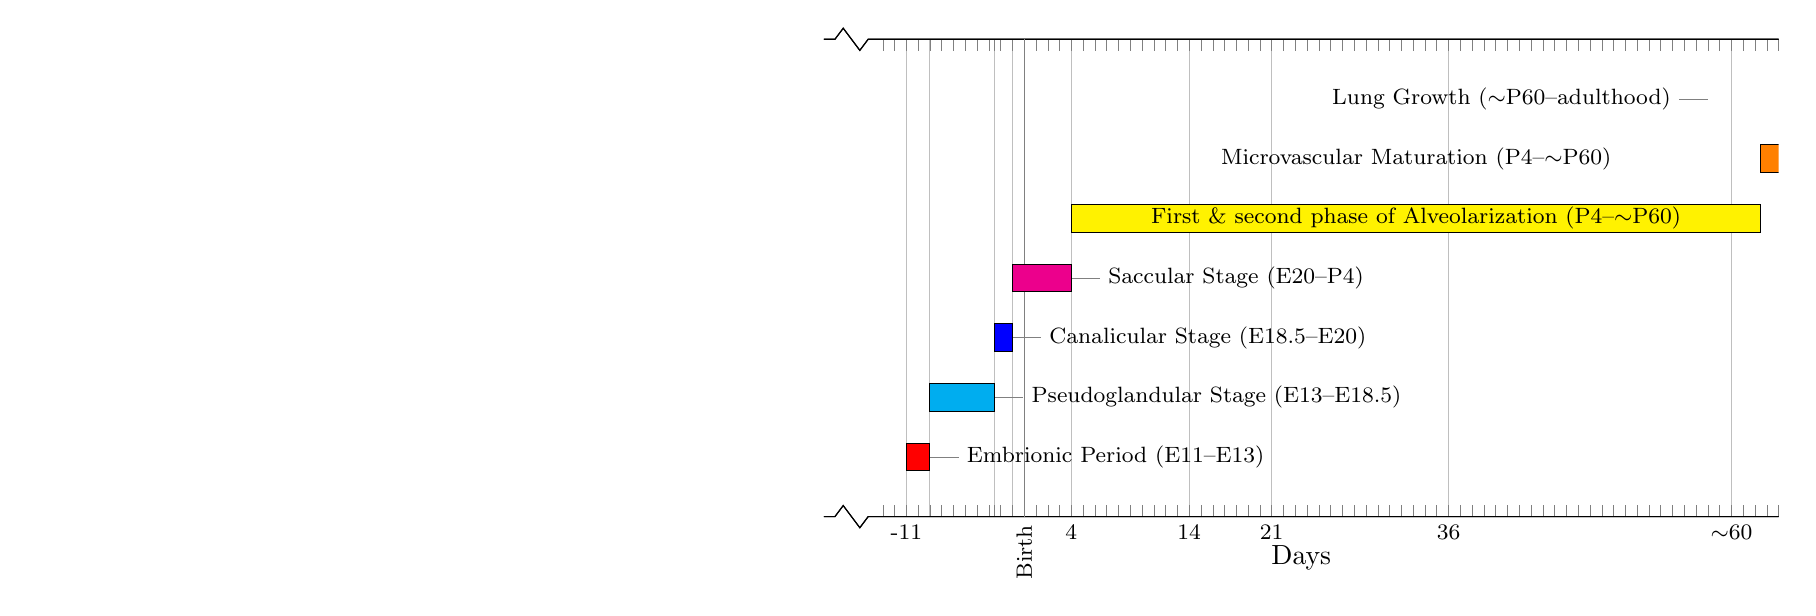
\begin{tikzpicture}
	\pgfplotsset{width=\linewidth,height=.5\linewidth}
		\def\xmin{4}
		\def\xmax{85}
		\def\ymin{0}
		\def\ymax{0.4}
		\def\step{0.05}
		\begin{axis}[xbar stacked,%
			scale only axis,%
			xmin=\xmin,xmax=\xmax,%
			ymin=\ymin,ymax=\ymax,%
			yticklabels={},%
			axis x discontinuity=crunch,%
			xtick={9,...,\xmax},%
			xticklabels={},
			xlabel=Days,%
			axis y line=none]
		\end{axis}
		\begin{axis}[xbar stacked,%
			scale only axis,%
			xmin=\xmin,xmax=\xmax,%
			ymin=\ymin,ymax=\ymax,%
			yticklabels={},%
			axis x discontinuity=crunch,%
			xtick={11,13,18.5,20,21,25,35,42,57,81},%
			xticklabels={-11,,,,,4,14,21,36,$\sim$60},
			xmajorgrids,%
			extra x ticks={21},%
			extra x tick style={major tick length=5cm,%
				tick label	style={	rotate=90,anchor=east}},%
			extra x tick labels={Birth},%
			axis y line=none]
			%\node [font=\footnotesize] at (axis cs:25,0.25) {X};
			%\node [font=\footnotesize] at (axis cs:83.5,0.25) {X};
			\node [font=\footnotesize] at (axis cs:54.25,0.25) {First \& second phase of Alveolarization (P4--$\sim$P60)};
			\node [font=\footnotesize] at (axis cs:54.25,0.3) {Microvascular Maturation (P4--$\sim$P60)};
			\def\step{0.05}
			\addplot [transparent]	coordinates {(11,0)};
			\addplot [fill=red]		coordinates {(2,1*\step)};
			\addplot [fill=cyan]		coordinates {(5.5,2*\step)};
			\addplot [fill=blue]		coordinates {(1.5,3*\step)};
			\addplot [fill=magenta]	coordinates {(5,4*\step)};
			\addplot [fill=yellow]	coordinates {(58.5,5*\step)};
			\addplot [transparent]	coordinates {(-58.5,5.5*\step)};
			\addplot [fill=orange]	coordinates {(58.5,6*\step)};
			\addplot [transparent]	coordinates {(-5,6.5*\step)};
			\addplot [fill=green]		coordinates {(\xmax-77,7*\step)};
			%\tikzstyle{every pin}=[%
				%fill=white,%
				%semitransparent,%
				%draw=black,%
				%text width=10em,%
				font=\footnotesize,
				%text centered,%
				pin distance=3ex]
			\node[coordinate, pin=right:{Embrionic Period (E11--E13)}] at (axis cs:13,0.05) {};
			\node[coordinate, pin=right:{Pseudoglandular Stage (E13--E18.5)}] at (axis cs:18.5,0.1) {};
			\node[coordinate, pin=right:{Canalicular Stage (E18.5--E20)}] at (axis cs:20,0.15) {};
			\node[coordinate, pin=right:{Saccular Stage (E20--P4)}] at (axis cs:25,0.2) {};
			\node[coordinate, pin=left:{Lung Growth ($\sim$P60--adulthood)}] at (axis cs:79,0.35) {};
		\end{axis}
	\end{tikzpicture}%
%%%%%%%%%%%%%%%%%%%%%%%%%%%%%%%%%%%%%%%%%%%%%%%%%%%%%%%%%%%%%%
%\end{document}